\thispagestyle{fancy}
\vspace*{\fill}
\subsection{Tela comando impressora}
 Esta tela é acessada pelo botão "\textgreater" no menu superior esquerdo da tela de comando alimentação, no mesmo botão da tela de comando das
\textbf{impressoras} ou no mesmo da tela comandos de uma impressora anterior (se ouver), pelo botão "\textless{}" no menu superior esquerdo da tela comando impressora posterior (se ouver) ou slotter quando não tiver nenhuma impressora a mais, pelo atalho na tela de comando das \textbf{impressoras} e pelo botão comando da tela ajustes impressora.
\begin{figure}[h]
  \centering
  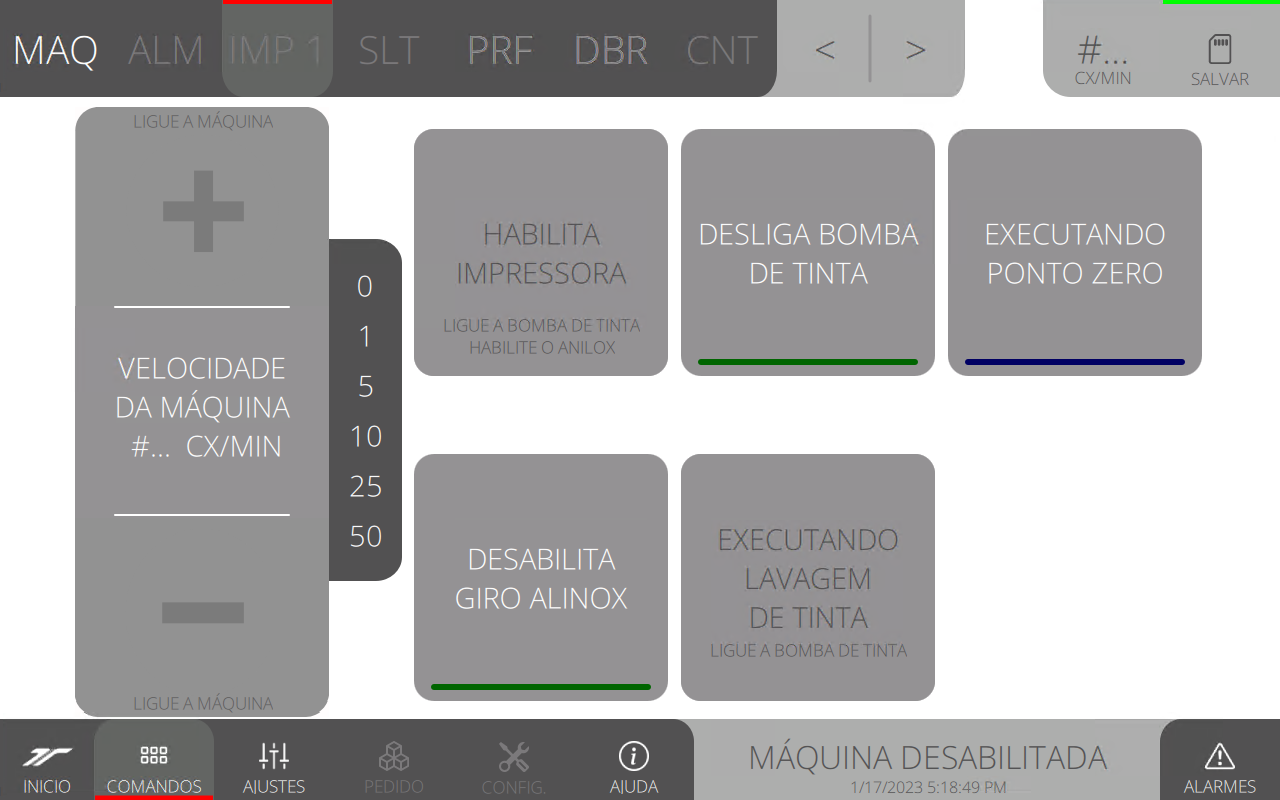
\includegraphics[width=576px,height=360px]{src/imagesFlexo/04-printter/02-printter/commands/e-Tela-Principal.png}
  \caption{ver depois.}
   \label{}
\end{figure}

\newpage
\thispagestyle{fancy}
\vspace*{\fill}
\subsubsection{\small{Executa lavagem de tinta}}
\begin{figure}[h]
  \centering
  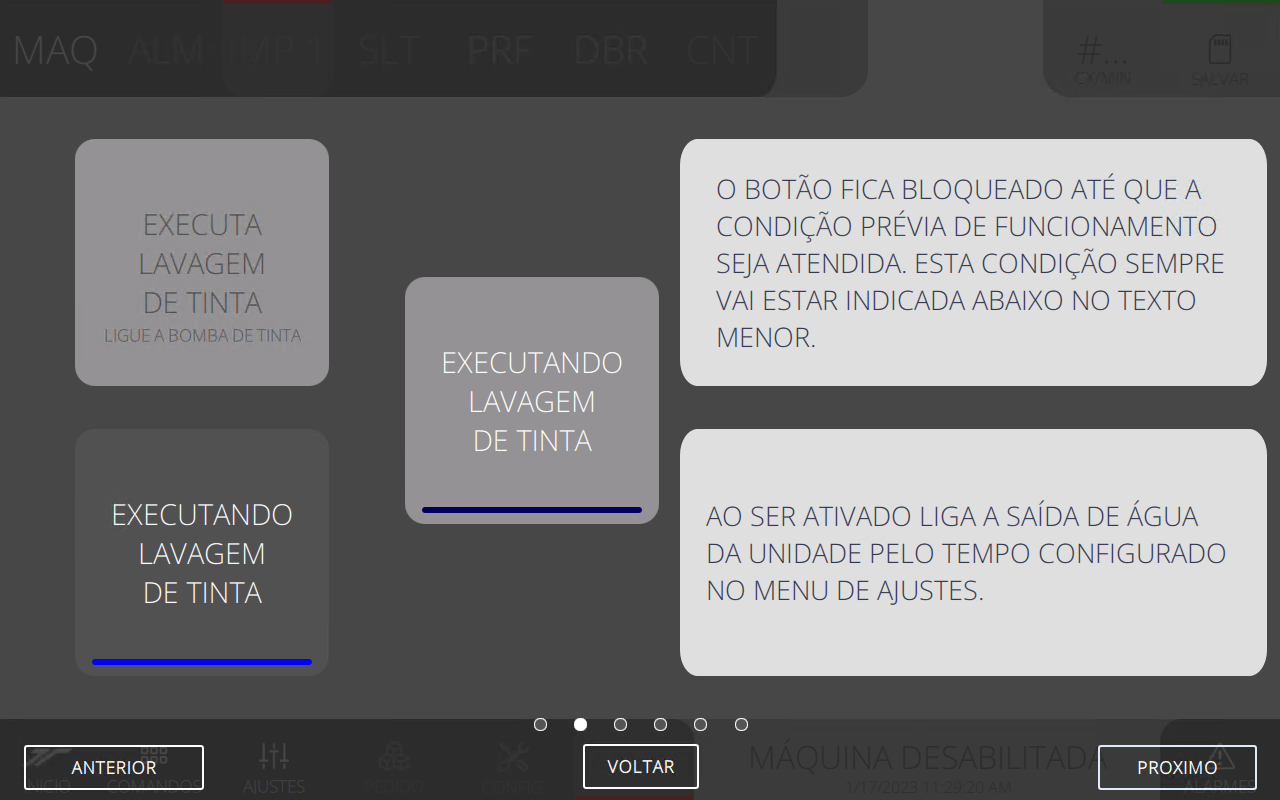
\includegraphics[width=576px,height=360px]{src/imagesFlexo/04-printter/02-printter/commands/e-2.png}
  \caption{ver depois.}
   \label{}
\end{figure}
\vspace*{\fill}

\newpage
\thispagestyle{fancy}
\vspace*{\fill}
\subsubsection{\small{Habilita giro anilox}}
\begin{figure}[h]
  \centering
  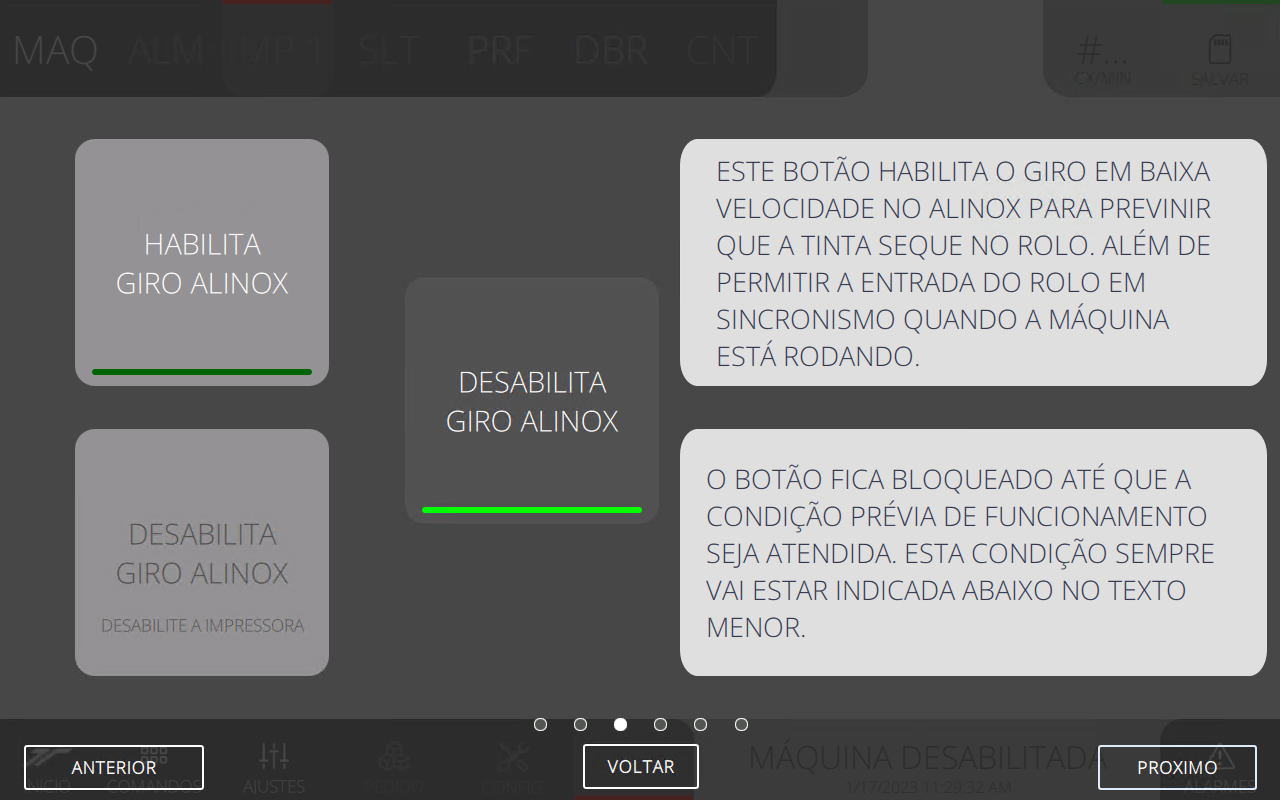
\includegraphics[width=576px,height=360px]{src/imagesFlexo/04-printter/02-printter/commands/e-3.png}
  \caption{ver depois.}
   \label{}
\end{figure}
\vspace*{\fill}

\newpage
\thispagestyle{fancy}
\vspace*{\fill}
\subsubsection{\small{Executa ponto zero}}
\begin{figure}[h]
  \centering
  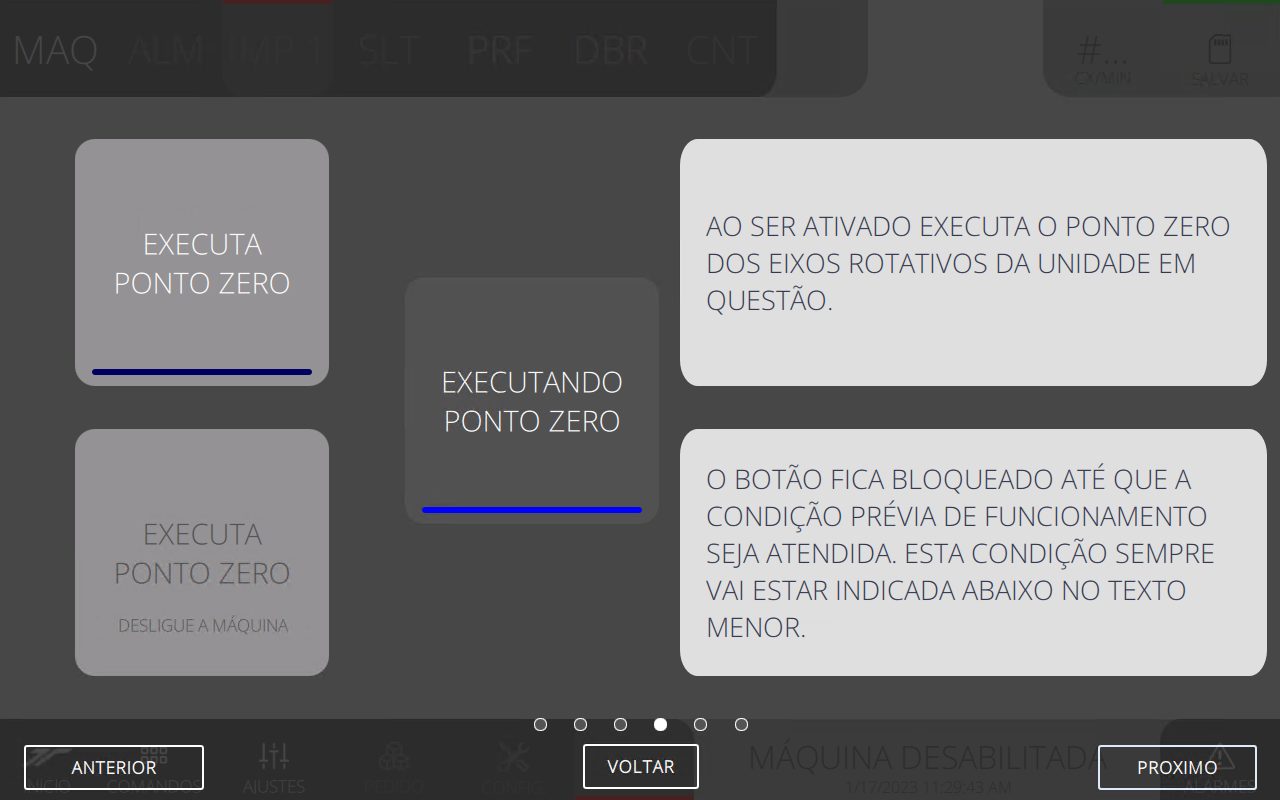
\includegraphics[width=576px,height=360px]{src/imagesFlexo/04-printter/02-printter/commands/e-4.png}
  \caption{ver depois.}
   \label{}
\end{figure}
\vspace*{\fill}

\newpage
\thispagestyle{fancy}
\vspace*{\fill}
\subsubsection{\small{Liga bomba de tinta}}
\begin{figure}[h]
  \centering
  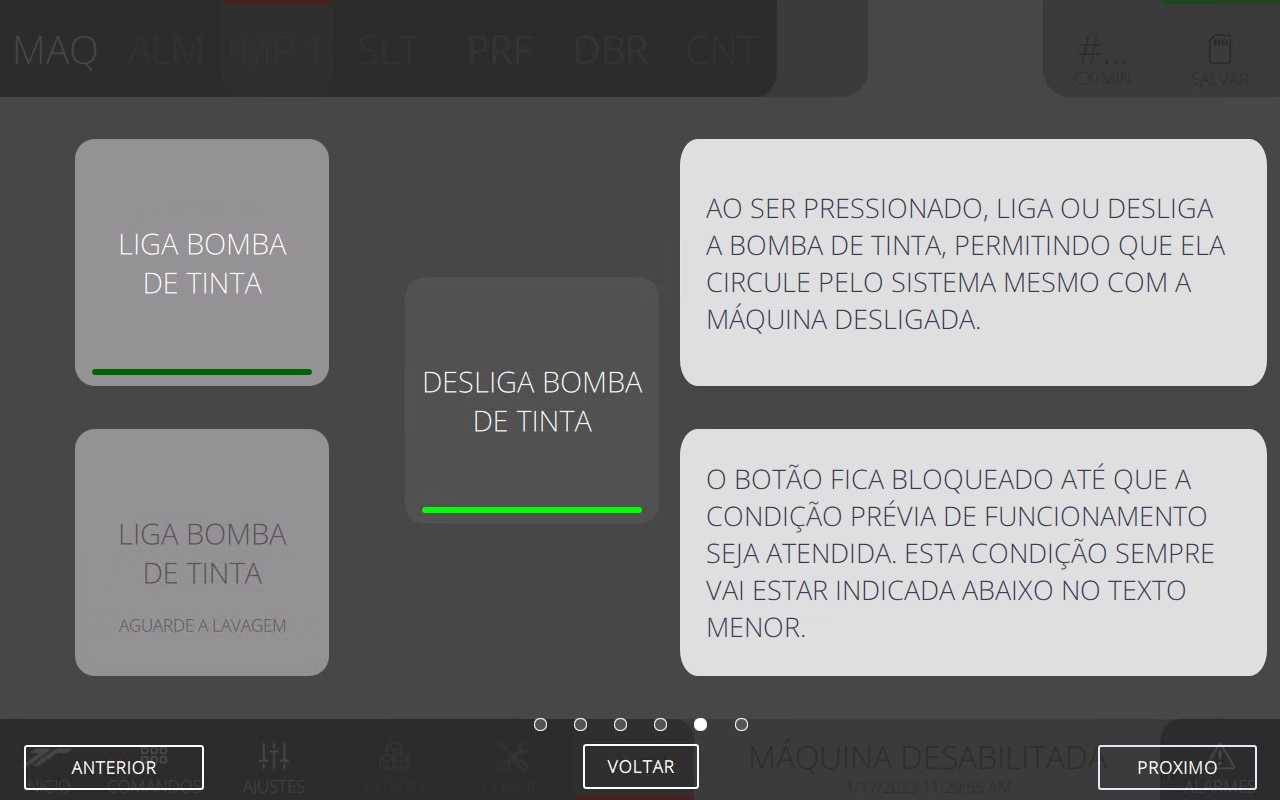
\includegraphics[width=576px,height=360px]{src/imagesFlexo/04-printter/02-printter/commands/e-5.png}
  \caption{ver depois.}
   \label{}
\end{figure}
\vspace*{\fill}

\newpage
\thispagestyle{fancy}
\vspace*{\fill}
\subsubsection{\small{Desabilita impressora}}
\begin{figure}[h]
  \centering
  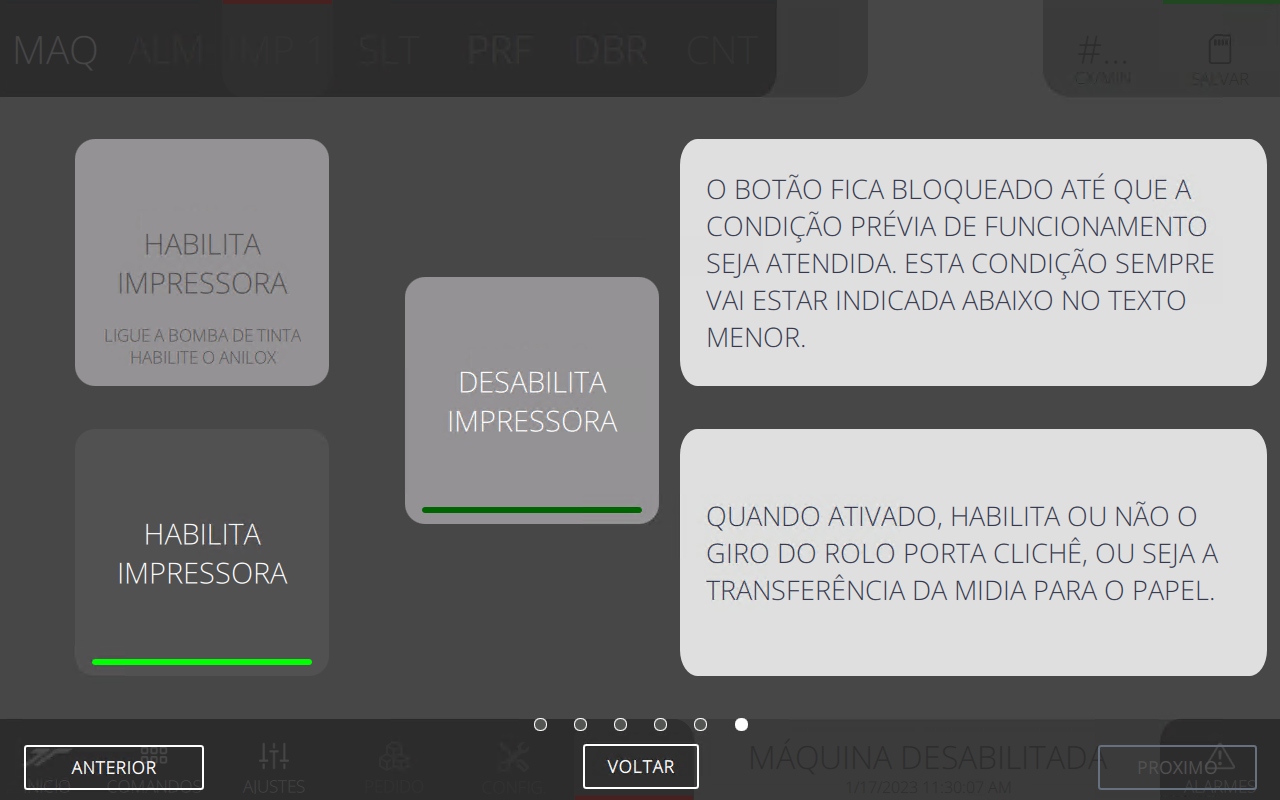
\includegraphics[width=576px,height=360px]{src/imagesFlexo/04-printter/02-printter/commands/e-6.png}
  \caption{ver depois.}
   \label{}
\end{figure}
\vspace*{\fill}